\chapter{Proposed Methodology}
\setcounter{equation}{0}

\nomenclature{DL}{Deep Learning}
\nomenclature{2D}{2-dimensional}
\nomenclature{ROM}{Read Only Memory}
\nomenclature{RAM}{Random Access Memory}
\nomenclature{GPU}{Graphics Processing Unit}
\nomenclature{VRAM}{Video RAM}
\nomenclature{OOM}{Out-Of-Memory}
\nomenclature{CSV}{Comma Separated File}

\section{Introduction}

With this project, the team attempts to create a robust violence detection system for video streams using deep learning techniques. This holds significant potential for enhancing public safety and security in various environments, including surveillance, law enforcement, and crowd monitoring. The proposed model combines spatial and temporal feature extraction methods into the system aiming to improve accuracy and automate the detection process.


% An automated violence detection system can offer valuable insights and enable prompt responses to potential threats, thereby contributing to the overall safety and well-being of communities.


% \section{Overview of the Proposed System}

% The envisioned system represents a pioneering advancement in the realm of public safety, offering a comprehensive solution for the automated detection and classification of violent incidents. Traditional methods for violence detection often rely on manual monitoring or human intervention, which can be labor-intensive, time-consuming, and prone to errors. With the advent of deep learning and computer vision techniques, there has been a paradigm shift towards automated approaches for violence detection in video streams. These methods leverage advanced neural network architectures to extract spatial and temporal features from video data and classify them into predefined categories, such as violent or non-violent.

% In this context, this project aims to develop an advanced violence detection system using deep learning techniques. The proposed system employs a combination of spatial and temporal feature extraction methods to enhance the accuracy and robustness of violence detection in video streams. By integrating state-of-the-art neural network architectures, including Convolutional Neural Networks (CNNs), Long Short-Term Memory (LSTM) networks, and attention mechanisms, the model can effectively capture both spatial and temporal patterns indicative of violent behavior. 

% The project focuses on the design and implementation of a comprehensive methodology for violence detection, encompassing frame extraction, preprocessing, feature extraction, and classification. Each step in the pipeline is carefully optimized to ensure efficient processing of video data while preserving essential spatial and temporal information. Additionally, advanced techniques such as data augmentation, normalization, and attention mechanisms are employed to improve the model's performance and generalization capabilities.

% Through sophisticated image processing techniques and machine learning models, the system can accurately discern the presence of violent behavior within monitored environments. By automating the process of identifying and categorizing violent incidents, the system significantly enhances situational awareness and empowers security personnel with actionable intelligence in real-time.

\section{Data Collection}

\noindent Effective violence detection systems rely on high-quality data for training and evaluation purposes. The process of collecting and curating data for violence detection entails several key considerations, including dataset size, diversity, and ethical considerations. In this section, an overview of the data collection methodology employed in violence detection research is explained.

\noindent Data collection begins with the identification of relevant sources, including surveillance videos, movies, television shows, and online platforms. Various sources were identified and researched to obtain the most suitable dataset for the best performance of the Model. The team embarked on a mission to enrich the dataset by staging meticulously choreographed violent scenes\cite{Recorded_violence}, which were then recorded to inject diversity into the dataset. Additionally, the team meticulously combed through CCTV footage\cite{Violent_flows} from various locations, including the college premises and neighboring shops and hotels, in search of real-life instances of violence with the intention of a violence detection framework that solely relies on visual features, eliminating the need for audio input \cite{audio_visual}\cite{ourdataset}. However, despite the efforts, the dataset obtained fell short in size, revealing the need for alternative approaches to expand it.

\noindent Efforts were made to stage violent scenes like collection of videos in \cite{kineticData} involving team members but encountered challenges due to the constraints posed by costumes, particularly the college uniform, which hindered the accurate identification of individuals and detection of their actions. This made the team shift its strategy towards exploring data available online. Thus, the team navigated through various avenues, adapting their approach to overcome obstacles and ensure the dataset's adequacy for training the model. Public datasets were the most favorable option, as they offered a wide range of data samples from diverse sources, ensuring a comprehensive representation of real-world scenarios for training the model.

\noindent In the publicly available datasets, several datasets can meet the violence detection process standards, but only a few can perform well. This is due to the scarcity of such datasets with proper labels for a systematic supervised learning algorithm. Here are some of the popular datasets:

\vspace{-5mm}

\begin{enumerate}
    \item \textbf{UCF-Crime Dataset:}
    The UCF-Crime dataset contains various types of violent and non-violent criminal activities captured from surveillance videos. It includes over 13,000 video clips annotated with violence labels, making it a valuable resource for violence detection and action recognition research. The content of this dataset is shown in Figure \ref{ucfcontent}. \\
    
    \begin{figure}[htbp!]
         \centering
         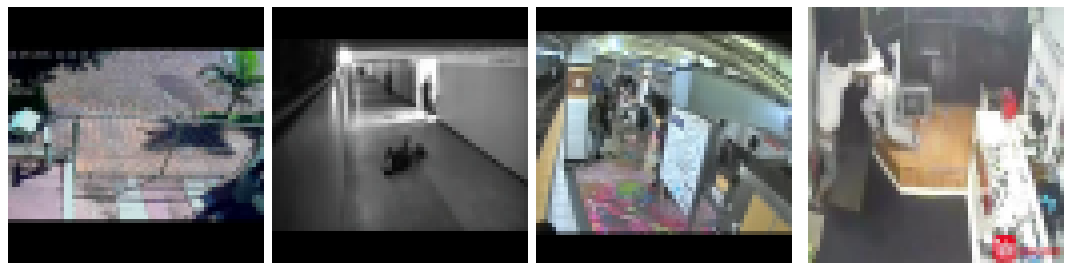
\includegraphics[width=1\linewidth]{Images/UCF.png}
        \caption{Contents of UCF-Crime Dataset}
        \label{ucfcontent}
    \end{figure}
    
\noindent Some challenges faced by this dataset are:
    \begin{itemize}
        \item The dataset primarily consists of surveillance videos capturing criminal activities, which may not adequately represent the diversity of public violence scenarios.
        \item This dataset is designed for general anomaly detection whereas anomalies in action may or may not include violent activities.
        \item The dataset may suffer from imbalanced class distributions, with a higher prevalence of non-violent activities compared to violent ones. 
        \item Videos in this dataset have a duration of up to 10 minutes, Hence, detecting violent activities from a long video is very difficult \cite{ourdataset} \\
    \end{itemize}

    \item \textbf{Movie Dataset:}
    The Movie Dataset is a collection of video clips extracted from movies, providing researchers with a diverse range of visual content for various applications, including violence detection. While this dataset offers rich and varied scenes depicting a wide array of actions and behaviors, including violent and non-violent interactions, it also presents several challenges for violence detection research:
       

    \begin{itemize}
        \item Movies span a wide range of visual content with varying levels of violence. Models must be robust enough to detect violent actions across different contexts and styles.
        \item The dataset may contain scenes with varying levels of resolution, lighting conditions, artificial elements, and camera viewpoints, impacting the visual representation of violent actions in the real world
        \item The Movies dataset may possess copyright issues with data being extracted from movies and may require the expenditure of money for alleviating copyrights.
    \end{itemize}\

    \item \textbf{Hockey Fight Dataset:}
    The Hockey Fight Dataset is a curated collection of video clips extracted from hockey games, specifically focusing on instances of fights between players\cite{hockey}. These clips are annotated to indicate the presence or absence of fights for research in violence detection and action recognition. The overview of the Hockey Fight dataset is given in Figure \ref{hockeyfight}.\\
    
    \begin{figure}[h]
        \centering
         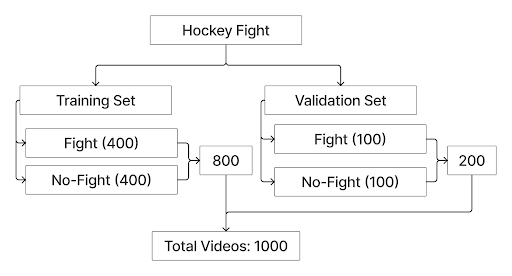
\includegraphics[width=0.9\linewidth]{Images/Hockey fight.png}
        \caption{Hockey Fight Dataset Overview}
        \label{hockeyfight}
    \end{figure}
    Here are some of the advantages of the Hockey Fight Dataset.


    \begin{itemize}
        \item The white color in the background of the hockey dataset videos likely provides a clear contrast with the players and other objects in the scene. This facilitates background separation, making it easier to isolate and track the players' movements and actions accurately.
        \item The compact nature of the hockey dataset, consisting of 1000 videos, offers several advantages for research and analysis. Despite its relatively small size compared to larger datasets, it remains valuable due to its focused scope and curated content.
        \item High-quality video recordings with clear resolution and minimal motion blur ensure that the players' movements are captured accurately, enhance the interpretability of the dataset, visualization of player actions, such as skating, passing, shooting, and defending, 
    \end{itemize}
    

     Nonetheless, this dataset also has some drawbacks including a lack of diversity of videos\cite{ourdataset}, Variability of duration, intensity, and multiple number of participants, which make it harder for algorithms to extract useful information.

    \item \textbf{RWF-2000 Dataset:}
    The RWF-2000 dataset is a widely used benchmark dataset for action recognition and violence detection research. It contains video clips extracted from movies, television shows, and YouTube videos, depicting various types of violent and non-violent behaviors. The dataset consists of 2,000 video clips, with 1600 clips used in the training set, 800 videos each for class Fight and Non-Fight, and the remaining 400 used in the validation set, 200 videos each for class Fight and Non-Fight \cite{ourdataset}. This dataset, whose overview and contents are displayed in Figure \ref{rwf2000overview} and Figure \ref{rwf2000content} respectively, showed superior performance when it comes to the detection of violence properly and accurately.
    %clearpage
    
    \begin{figure}[h!]
        \centering
        \includegraphics[width=0.9\linewidth]{Images/rwf_content.png}
        \caption{Contents of RWF-2000 Dataset}
        \label{rwf2000content}
    \end{figure}

%\clearpage
    
    % The RWF-2000 dataset stands out as a superior resource for violence detection research due to several key factors that are mentioned later. This dataset has emerged as the most suitable dataset for the intended purpose.\\

    \begin{figure}[h!]
        \centering
        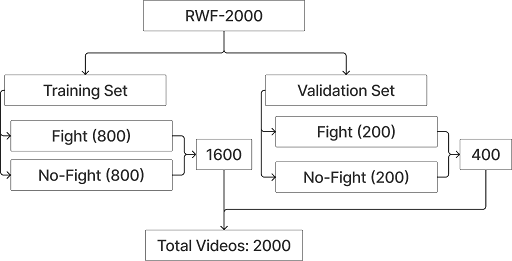
\includegraphics[width=0.9\linewidth]{Images/RWF_Dataset.png}
        \caption{RWF-2000 Dataset Overview}
        \label{rwf2000overview}
    \end{figure}

% \clearpage

    Some of the advantages of RWF-2000 over other datasets for violence detection are in Table \ref{rwf2000adv} and Table \ref{rwf2000disadv}.
    
    % \begin{itemize}
    %     \item With over 2,000 video clips, the RWF-2000 dataset offers a substantial collection of data for training and evaluating violence detection algorithms. This large dataset size enables models to generalize well across diverse scenarios and contexts
    %     \item Each video clip in the RWF-2000 dataset is comprised of 150  frames (30fps  x 5 sec) making it of equal duration and similar size. This ensures that each video clip is balanced and the whole dataset has been limited to 2000x150 frames. 
    %     \item This dataset is also labeled with an equal split for both the classes containing 1000 clips each for the Fight and Non-Fight classes preventing class imbalances.
    %     \item The Dataset is arranged with a train-test split of 80\% training data (1600 samples) and 20\% testing data (400 samples), it is an ideal range for optimal performance results
    %     \item The RWF-2000 dataset is a widely used benchmark for violence detection research, serving as a standard reference point for evaluating the performance of different algorithms and technique
    % \end{itemize}

\vspace{1cm}

\begin{table}[h!]
\centering
\caption{Advantages of RWF-2000 Dataset}
\begin{tabular}{|c|p{12cm}|}
\hline
\textbf{No.} & \textbf{Feature}                                                                                                        \\ \hline
1            & The RWF-2000 dataset contains over 2,000 video clips, providing a substantial volume of data for training and evaluation. \\ \hline
2            & Each video clip consists of 150 frames (30fps x 5 sec), ensuring equal duration and size across the dataset.              \\ \hline
3            & The dataset is balanced with 1000 clips each for Fight and Non-Fight classes, avoiding class imbalances.                  \\ \hline
4            & Arranged with an 80\% train (1600 samples) and 20\% test (400 samples) split, ideal for optimal training and testing.     \\ \hline
5            & Widely recognized as a benchmark in violence detection research, it serves as a standard reference for algorithm evaluation. \\ \hline
\end{tabular}
\label{rwf2000adv}
\end{table}

\clearpage
\noindent The resolution distribution of the RWF-2000 dataset is given in Figure \ref{rwf2000resolutiondist}.    

\begin{figure}[h!]
\centering
    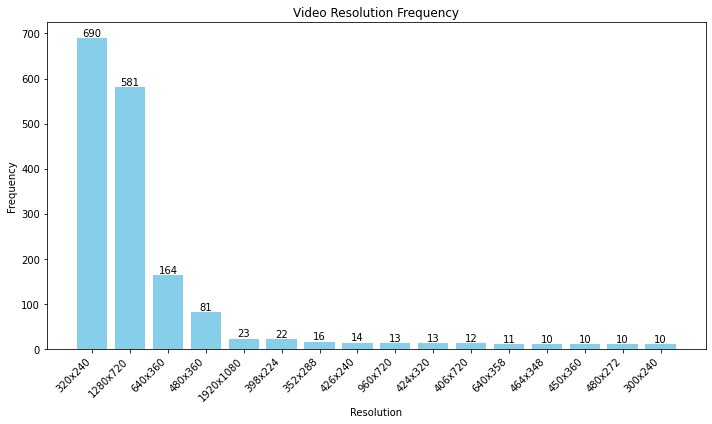
\includegraphics[width=0.8\linewidth]{Images/RWF-2000 Video Resolution freq bar plot.png}
    \caption{RWF-2000 Video Resolution Distribution}
    \label{rwf2000resolutiondist}
\end{figure}


% To address limitations such as low image quality, insufficient data quantity, videos with long durations but crude annotations, and hybrid sources merely resembling any realistic violence, RWF-2000  \cite{ourdataset}  emerged as the useful dataset for computer vision tasks. along with the Hockey Fight dataset which became important later on during the project development phase.
\end{enumerate}

\vspace{-5mm}

\begin{table}[h!]
\centering
\caption{Disadvantages of RWF-2000 Dataset}
\begin{tabular}{|c|p{12cm}|}
\hline
\textbf{No.} & \textbf{Disadvantage}                                                                                          \\ \hline
1            & Quality from YouTube varies widely, introducing inconsistencies that can affect model performance.              \\ \hline
2            & Use of specific keywords may miss some types of violence, leading to a biased dataset.                          \\ \hline
3            & Videos of real people used without consent raise ethical concerns and privacy issues.                           \\ \hline
4            & Models may overfit the types of violence in the dataset and won't generalize well.                             \\ \hline
5            & Lack of contextual information can make it difficult to distinguish between real and staged violence.           \\ \hline
6            & Potential legal issues related to copyright when using YouTube videos for research or commercial purposes.      \\ \hline
7            & Inaccuracies in video labeling can mislead training and affect detection system performance.                    \\ \hline
\end{tabular}
\label{rwf2000disadv}
\end{table}



% ----------------------------------------------------

\clearpage

\section{Dataset Preprocessing}

The Preprocessing begins with the transformation of raw video data, which undergoes initial preprocessing steps to enhance interpretability and facilitate downstream analysis. The data preprocessing encompasses the following steps:

\begin{itemize}
    \item Renaming the videos based on their content, such as labeling fight-related videos as "Fight\_1..." and "No\_Fight\_1...," for videos with no fight, which ensures better organization and understanding of the dataset. 

    \item Subsequently, the videos are subjected to frame extraction that decomposes the continuous video stream into individual frames. Each video's frames are then saved in a corresponding folder, named after the original video, simplifying data management and retrieval as shown in Figure \ref{processnormal}.
    

    \item Following frame extraction, the frames undergo resizing to a standardized format of 224x224 pixels with three color channels (224x224x3). This resizing ensures compatibility with most pre-trained deep learning models and facilitates efficient processing. While resizing maintains the essence of the video content, preserving three color channels balances the trade-off between training time, accuracy, and computational speed.

    \item Transforming data into the .npy format simplifies data management, data retrieval, and streamlining operations with efficient memory mapping. This optimization enhances read and write speeds, optimizing resource utilization for smoother training and inference processes.
\end{itemize}

    \noindent In the context of data handling, .npy files offer advantages over individual image files by consolidating multiple video frames into a single numpy array file. This simplifies the process of accessing and managing data, as users only need to interact with the .npy file instead of iterating through numerous image files placed inside different folders. The process of storing and searching in NumPy files is shown in Figure \ref{processnumpy}.\\

    \begin{figure}[h!]
        \centering
        
\includegraphics[width=1\linewidth]{Images/without npy.png}
        \caption{Storing and Searching in Normal Files}
        \label{processnormal}
    \end{figure}

    \begin{figure}[h!]
        \centering
        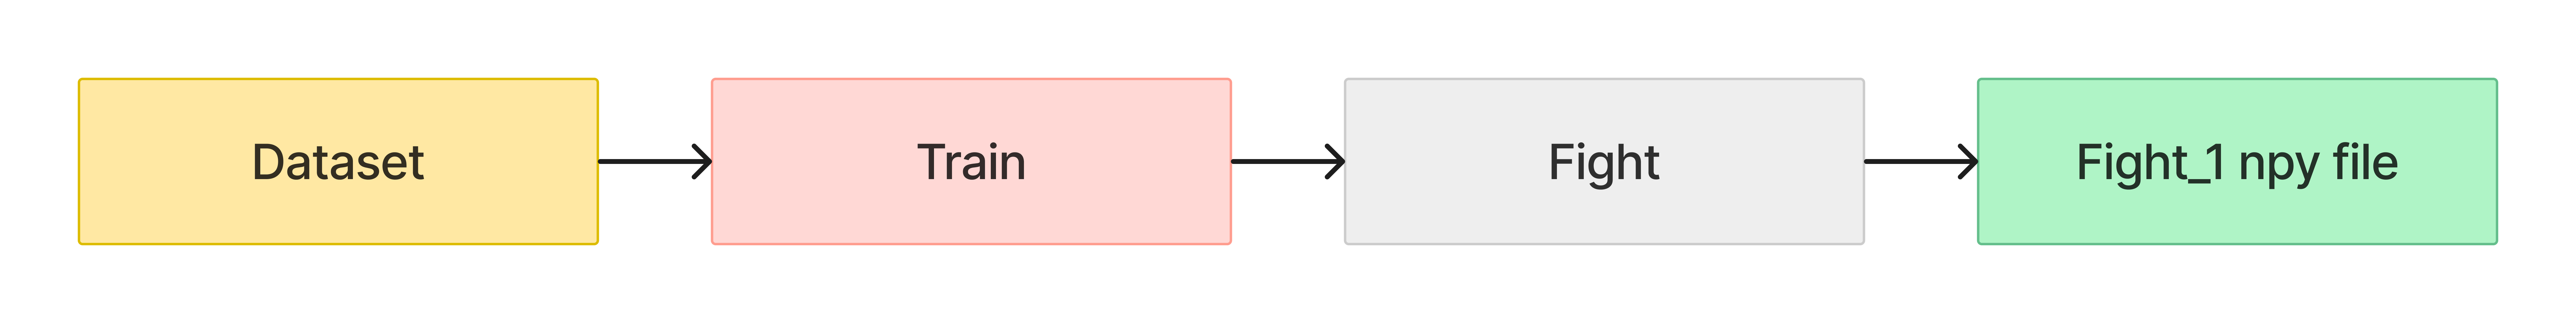
\includegraphics[width=1\linewidth]{Images/With npy.png}
        \caption{Storing and Searching in NumPy Files}
        \label{processnumpy}
    \end{figure}

    \noindent Moreover, .npy files are stored in a binary format, resulting in smaller file sizes compared to collections of image files, which further enhances efficiency during data manipulation and storage. Figure \ref{memorymap} shows how the memory is mapped as a path to these .npy files.
    
    \begin{figure}[h!]
        \centering
        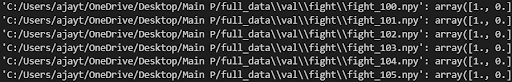
\includegraphics[width=0.9\linewidth]{Images/Mem map.png}
        \caption{Memory Mapping Printed as Path to the NumPy Files}
        \label{memorymap}
    \end{figure}

\noindent The combination of these preprocessing steps sets the stage for subsequent feature extraction and model training, enabling the development of a robust violence detection system. By transforming raw video data into a structured and standardized format, the project lays the foundation for effective analysis and interpretation. Additionally, the systematic organization of data enhances the scalability and reproducibility of the violence detection pipeline.

% ----------------------------------------------------

\clearpage

% \section{Model Building and Coding Practices}

% This section provides a detailed overview of the proposed system, outlining the technical procedures and methodologies used from initiation to completion, which includes descriptions of the model layers used, and the coding standards.

\section{Model Building}

% The proposed model was built to process videos sequentially, before the initial design of the model, the objectives were outlined clearly to make a model that is lightweight, fast, uses less computing, and is trainable in gaming laptops.

\begin{figure}[h!]
    \centering
    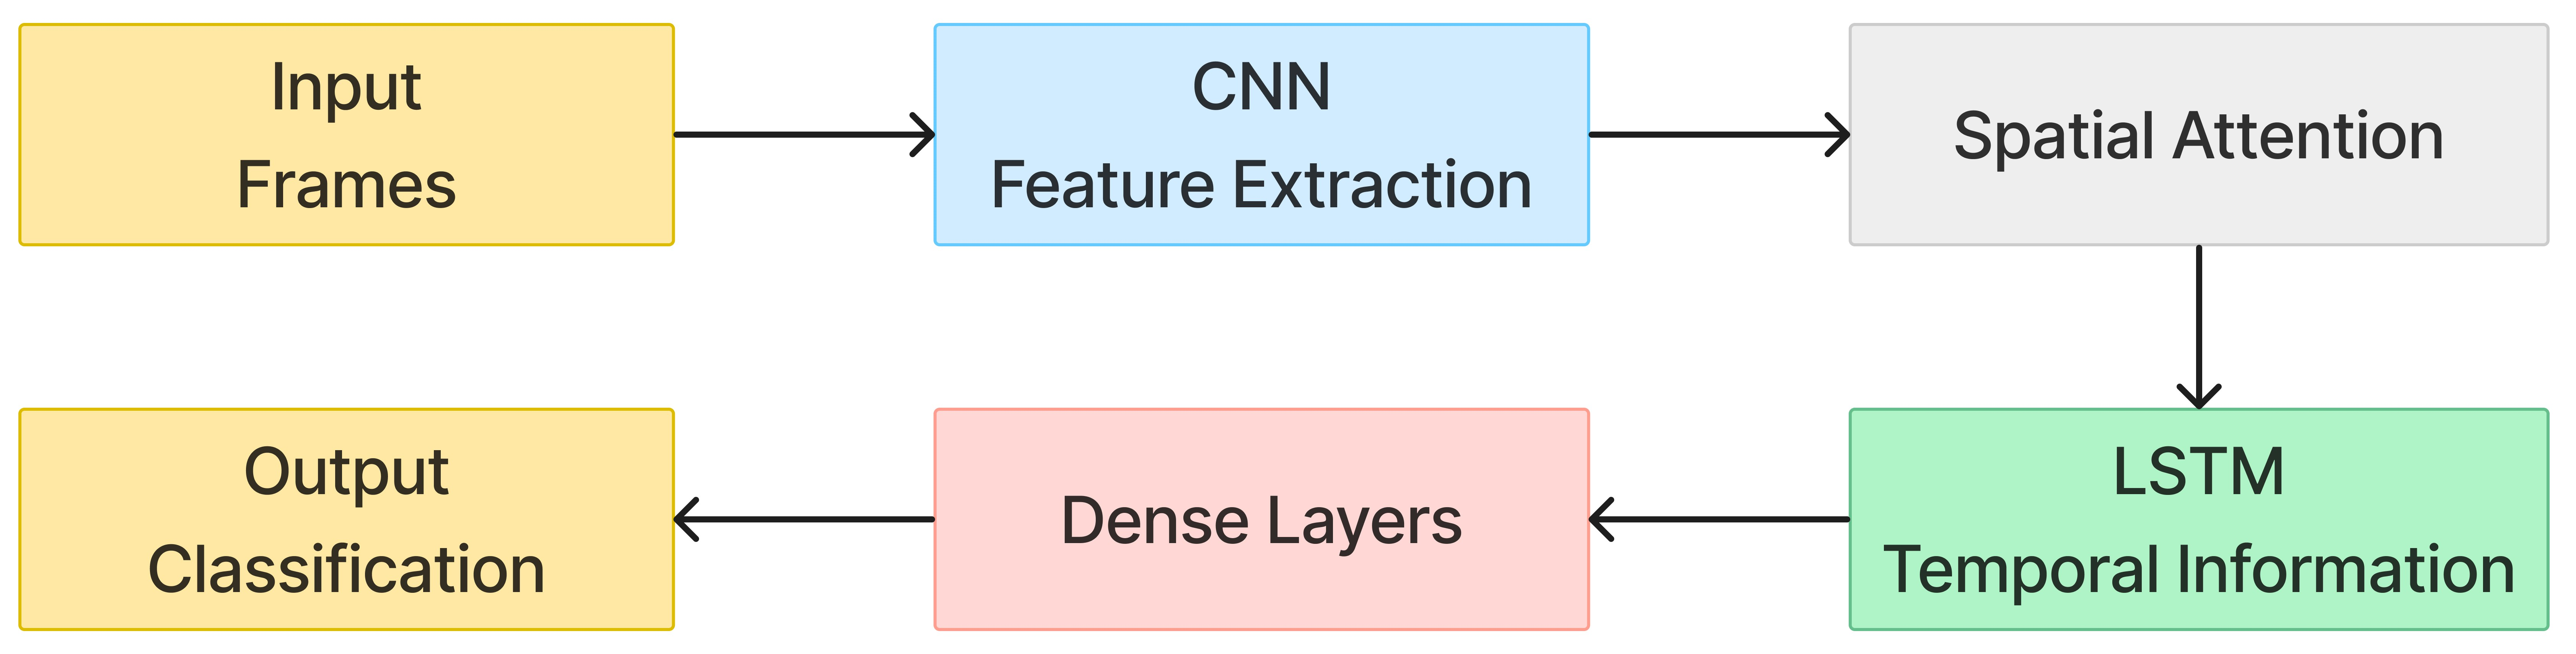
\includegraphics[width=0.9\linewidth]{Images/sys_high_level_overview.jpg}
    \caption{High-Level Overview of the Proposed System}\
    \label{fig:HighLevelOverview}
\end{figure}

\vspace{-5mm}

\noindent The design of the model started from a simple idea of \textit{how humans look and understand a violent situation}. Consider an example of a violent activity happening some distance away from a person, the person tends to focus on speech, disturbance, and movements. After some milliseconds the focus will be shifted to more detailed things in the view, like if a weapon is used, the emotional state of people surrounding the situation (anger, fear, and disgust) within a short duration of time the person will understand the situation and act accordingly. The team concentrated on building this type of response using deep learning methods, The initial focus of the person can be implemented using a special type of deep learning architecture called CNN which is an abstraction of human perception. To make the CNN focus on minute and detailed items present in the view the team used a simple attention mechanism called \textit{Spatial Attention}, which identifies the brightest(regions with high RGB values) and most averaged parts(repeated across many video frames, like quick movements) and makes a map out of it and compares with the original frames and returns the attended region which makes the important features stand out more during the network's learning process. But this Spatial Attention only helps to understand what is in a frame and where to focus. To act like a human, the network needs to know how the information changes over time, for this another deep learning architecture called LSTM was used. LSTMs are a type of 
Recurrent Neural Networks (RNN), that are designed to handle data in sequences. It has memory cells and other gates, which can maintain its state over time, effectively allowing the network to remember past information for an extended period. This is key to understanding temporal patterns and dependencies(time-based patterns).

\clearpage

\noindent Together CNN, Spatial Attention, and LSTM simulate the working of a human brain when the person is near a violent situation. But this can change with the situation (in technical terms, the data), as this biological response pattern is a general pattern for action recognition in humans, as for the proposed network architecture.


\noindent The high-level overview the proposed system consists of 6 different phases, each of which has a different deep learning architecture used. The diagrammatic representation of these phases can be seen in Figure \ref{fig:HighLevelOverview}. Details of each of these steps from data preprocessing to final output are described as follows.

% no clearpage here

\section{Detailed Description of the System}

\begin{figure}[!htbp]
    \centering
    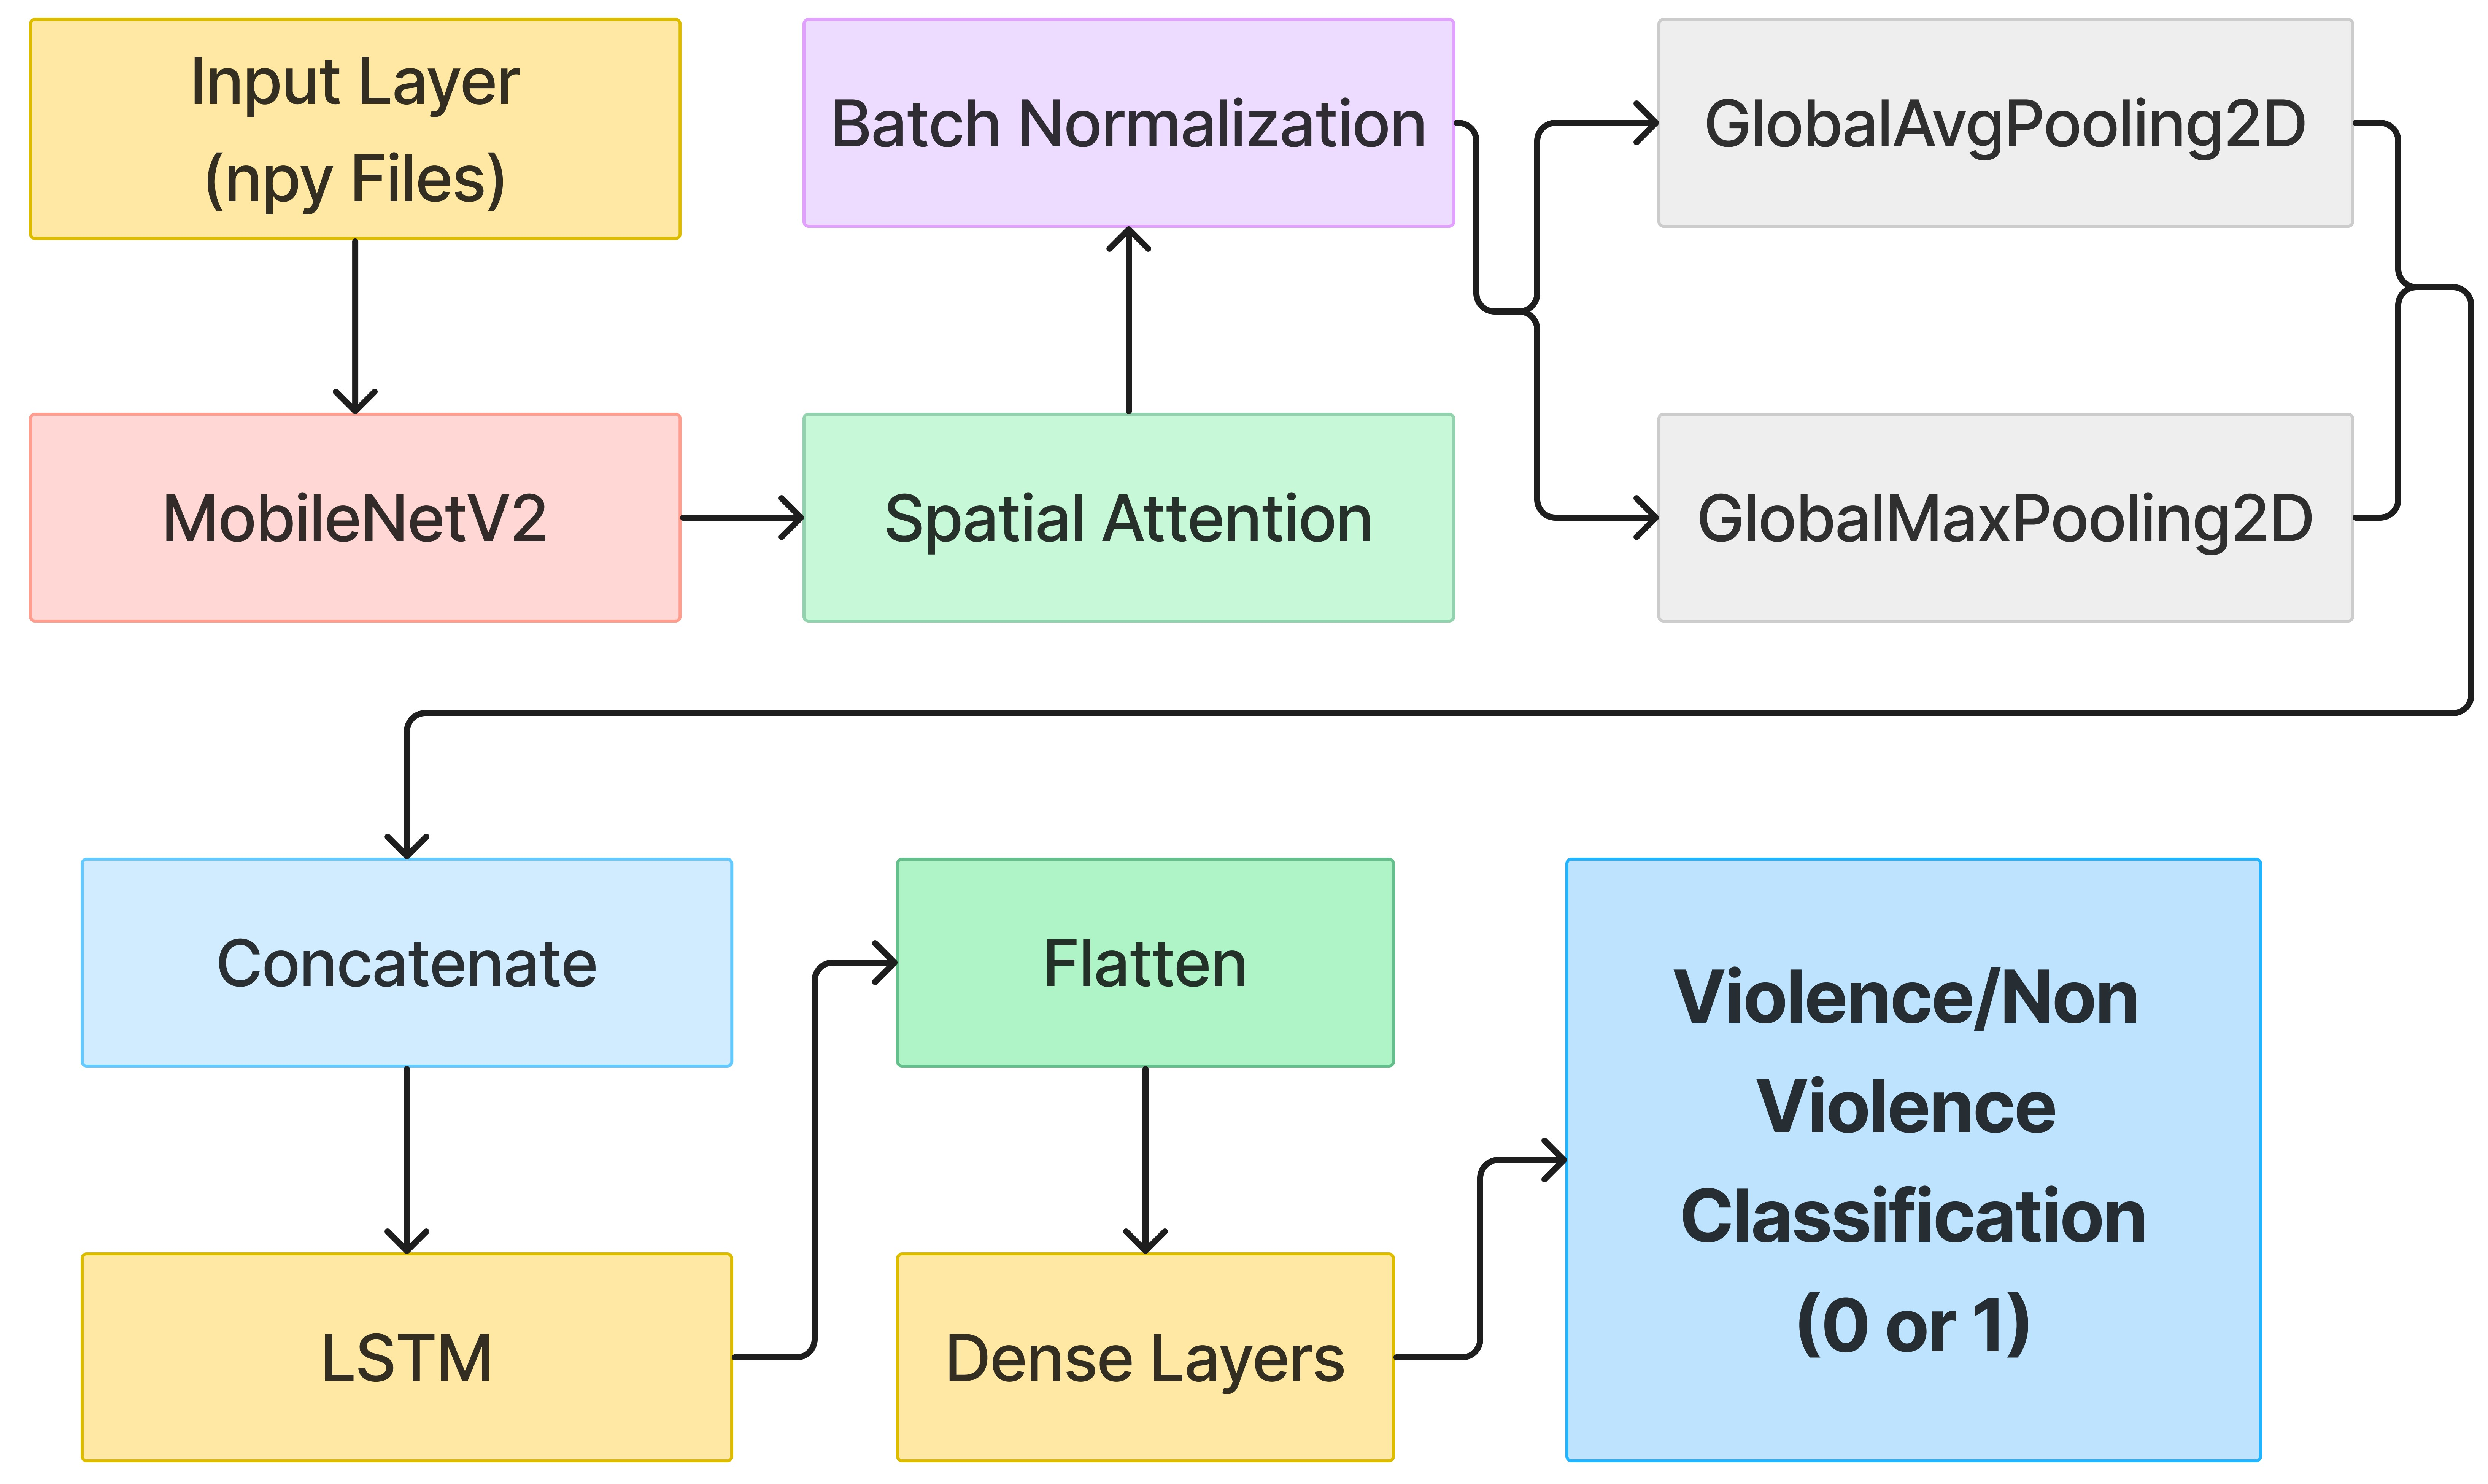
\includegraphics[width=0.74\linewidth]{Images/prop_sys.jpg}
    \caption{Block Diagram of the Proposed System}\
    \label{fig:BlockDiagram}
\end{figure}

\noindent Figure \ref{fig:BlockDiagram} shows the architecture of the proposed system which is a simple but effective model construction that consists of different components working together to classify whether a video contains violence or not. The approach is a single-stream approach where the data sequentially goes through each layer of the model.

\clearpage

\subsection{Frame Extraction and Sampling: }

\noindent The preprocessing pipeline for video input begins with frame extraction, breaking down continuous streams into individual frames for subsequent analysis. Converting videos into sequential frames enables processing at the frame level, essential for analysis by computer vision models, facilitating action recognition and event detection in video data.

\noindent Resizing these frames to a standardized 224x224x3 format enhances computational efficiency and accelerates learning processes while reducing complexity. Standardizing resolutions ensures consistency across the dataset, enabling models to learn invariant features and improving generalization performance on unseen data. 

\noindent Converting frames into NumPy's .npy format optimizes storage and access, leveraging the format's efficient binary representation for faster read and write operations than traditional image file formats. Converting to .npy format streamlines data handling, reducing complexity and enabling efficient memory mapping for faster read and write operations, optimizing resource utilization during training and testing.

\noindent To maintain temporal context while managing computational resources effectively, a uniform sampling strategy is employed. This approach involves selecting frames at regular intervals, ensuring a balance between computational efficiency and the retention of essential information.

% \noindent Furthermore, the preprocessing pipeline sets the stage for subsequent feature extraction, where spatial and temporal features are extracted to capture relevant information from individual frames and temporal sequences. These features serve as inputs to downstream violence detection algorithms, contributing to improved accuracy and robustness in identifying violent activities within video streams. Thus, the preprocessing steps play a crucial role in optimizing computational efficiency, preserving temporal context, and enhancing the overall effectiveness of violence detection systems.

\subsection{Feature Extractor CNN}

\noindent The rich representations inside each frame of a video will be captured by feature extraction CNN models, in this case, the team has used a lightweight and fast pre-trained model named MobileNetV2, which is designed for the implementation on edge devices and provides a quick output. It is suggested in \cite{renjith_sir_paper} that effectiveness and accuracy can be improved by the usage of pre-trained models. 

\clearpage

\noindent The MobileNets uses a special kind of CNN called Depthwise Separable Convolution, it has a minor change from traditional CNN, as it splits the computation into two steps: depthwise convolution and pointwise convolution, the first applies a single convolution filter to each of the input channel and the later is used to create a linearly combined output of the depthwise convolution, these actions reduce the total number of multiplications required in computation than a traditional CNN. In the proposed model the 20 layers on the bottom of MobileNet were frozen, as there is no need to train the model to capture high-level details like edges, bright spots, etc.

\noindent But going to the top all other layers are trainable because it is required to capture minute details present in video frames. All of these operations are done using a special kind of layers called TimeDistributed layers, which do the corresponding operations to all the frames passed to the network in a batch. The code implementation is given below.

\begin{lstlisting}
from tensorflow.keras.applications import MobileNetV2
base_model = MobileNetV2(include_top=False, weights='imagenet', input_shape=input_shape[1:])
base_model.trainable = True
for layer in base_model.layers[:-20]: # Freeze last 20 layers
    layer.trainable = False
frames_features = TimeDistributed(base_model)(inputs)
\end{lstlisting}

\vspace{-5mm}

\subsection{Spatial Attention Mechanism :}

\noindent The output of MobileNetV2 is a group of feature maps that contains the spatial and temporal dimensions. The Spatial Features \cite{Spacial_feat} extracted from video frames capture static information, while temporal features \cite{Spacio-tempo} represent dynamic changes over time. The model needs special attention towards the spatial information, to focus on important parts of the frames, they are passed through a Spatial Attention module. This helps the model to improve its ability to capture important visual features associated with violence. The spatial attention works in a simple manner, where the maximum and average values across the frame batch are calculated and concatenated along the channel axis. 

\noindent This is then passed through a single filter CNN to make an activation map(shown in results and discussions) having values between 0 and 1. Finally, a multiplication operation is done against the feature map with the original input tensor element-wise, this multiplication operation basically acts as a gating mechanism where values close to 1 in the attention map allow the corresponding features in the input tensor to pass, and values close to 0 will be blocked. The code used for spatial attention is given below.

% \clearpage

\begin{lstlisting}
class SpatialAttention(Layer):
    def __init__(self, **kwargs):
        super(SpatialAttention, self).__init__(**kwargs)

    def build(self, input_shape):
        self.conv2d = Conv2D(1, (7, 7), activation='sigmoid', padding='same')
        super(SpatialAttention, self).build(input_shape)

    def call(self, inputs):
        max_pool = tf.reduce_max(inputs, axis=-1, keepdims=True)
        avg_pool = tf.reduce_mean(inputs, axis=-1, keepdims=True)
        concat = Concatenate(axis=-1)([max_pool, avg_pool])
        attention = self.conv2d(concat)
        return Multiply()([inputs, attention])
\end{lstlisting}


\subsection{Batch Normalization:}

\noindent Following the spatial attention mechanism and learning in general the distribution of activations in each layer may shift, leading to slower convergence and degraded performance. Batch normalization is a useful technique that can be applied to stabilize the activations, which helps improve the convergence and training speed of the model.

\subsection{Feature Pooling \& Concatenation:}

The output from batch normalization is then split into two branches. One branch is dedicated to GlobalAveragePooling2D, and the other to GlobalMaxPooling2D. These pooling operations reduce the size of feature maps and output combined information about the features. The results from both pooling operations are concatenated to capture comprehensive spatial information from the video frames.

\subsection{LSTM Network:}

\noindent The concatenated feature vector resulting from the pooling operations is then inputted into an LSTM network. LSTM networks are a type of RNN specifically designed for modeling sequential data and are proficient at capturing temporal dependencies and long-term patterns within sequences. In the context of video analysis, LSTM enables the model to effectively encode temporal information and identify complex patterns that extend over multiple frames. This is made possible by the presence of memory cells and gating mechanisms inside the LSTM. 

\subsection{Dense Layer \& Classification:}
Following the LSTM layer, the output(2D Tensor) is flattened using a Flatten layer(to 1D vector) and is passed through a collection of dense layer with dropout layers fitted between them to prevent overfitting. The final dense layer is followed by a softmax activation function to classify the output into two classes: violence or non-violence(labelled as 'Fight' and 'No Fight').

\noindent The key layers or components of the proposed system with its important functions are listed below in Table \ref{propsysfunc}. The summary of the model architecture is shown in Table \ref{table:modelsummary} while the model definition generated using the Keras Plotting utility is shown in Figure \ref{KerasBlockDiagram}.

\clearpage

\begin{table}[!htbp]
\centering
\caption[Key Components of Proposed System]{Key Layers/Components of Proposed System with Functions and Importance}
\begin{tabular}{|>{\raggedright\arraybackslash}m{4cm}|>{\raggedright\arraybackslash}m{5cm}|>{\raggedright\arraybackslash}m{5cm}|}
\hline
\textbf{Layer/Component} & \textbf{Function} & \textbf{Importance} \\ \hline
Frame Extraction & Converts video into sequential frames. & Essential for analyzing actions frame by frame. \\ \hline
Frame Resizing & Standardizes frame size to 224x224x3. & Ensures uniform input dimensions for consistent processing. \\ \hline
NumPy Conversion (.npy) & Optimizes frame storage and access. & Enhances data handling speeds and training efficiency. \\ \hline
Uniform Sampling & Selects frames at regular intervals. & Balances computational load and info retention. \\ \hline
Feature Extractor CNN (MobileNetV2) & Extracts features using depthwise separable convolutions. & Extract spatial features within frames. \\ \hline
Spatial Attention Mechanism & Highlights important spatial features in frames. & Focuses model on significant areas, improving detection accuracy. \\ \hline
Batch Normalization & Stabilizes activations, improve training efficiency. & Ensures faster, more stable training convergence. \\ \hline
Feature Pooling \& Concatenation & Reduces dimensionality and combines features. & Captures comprehensive spatial information from frames. \\ \hline
LSTM Network & Captures temporal dependencies and patterns across frames. & Essential for recognizing sequences of actions that indicate violence. \\ \hline
Dense Layer \& Classification & Processes features to classify the video as 'violence' or 'non-violence'. & Makes the final decision using learned features to detect violent behavior. \\ \hline
\end{tabular}
\label{propsysfunc}
\end{table}

\clearpage

\begin{figure}[htbp!]
    \centering
    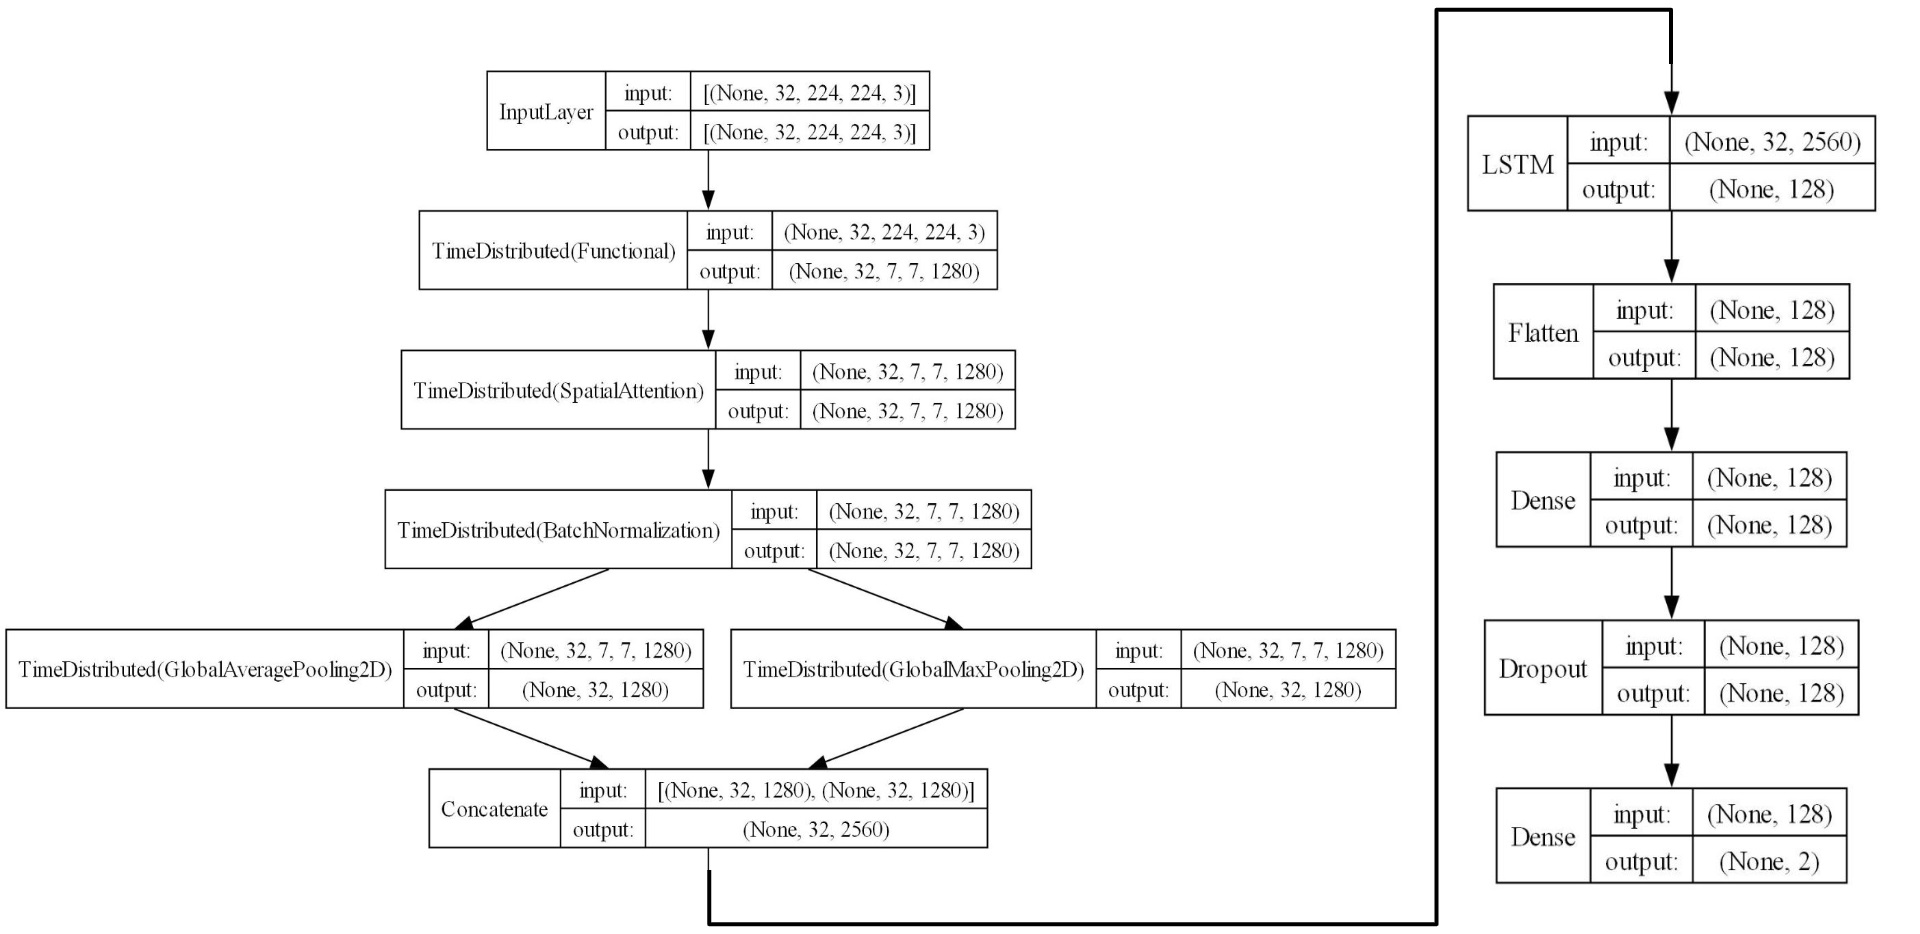
\includegraphics[width=0.99\linewidth]{Images/our_model.jpg}
    \caption{Keras Plotting Utility's Output of Model Definition in Code}\
    \label{KerasBlockDiagram}
\end{figure}

\vspace{-10mm}

\begin{table}[H]
\centering
% \caption[Summary of Model Architecture]{Summary of Model Architecture(*TimeDistributed $|$ Total Parameters: 3,659,990)}
\caption{Summary of Model Architecture}
\begin{tabular}{c|c|c|c}
\hline
\textbf{Layer (type)}            & \textbf{Output Shape}       & \textbf{Param \#} & \textbf{Connected to}               \\ \hline
input\_1 (InputLayer)            & (None, 20, 224, 224, 3)     & 0                 & []                                   \\ 
MobileNetV2* & (None, 20, 7, 7, 1280)      & 2,257,984         & ['input\_1[0][0]']                   \\ 
Spatial Attention* & (None, 20, 7, 7, 1280)      & 99                & MobileNetV2*         \\ 
Batch Normalization* & (None, 20, 7, 7, 1280)      & 5,120             & Spatial Attention*      \\
GlobalAveragePooling2D* & (None, 20, 1280)            & 0                 & Batch Normalization*    \\
GlobalMaxPooling2D* & (None, 20, 1280)            & 0                 & Batch Normalization*     \\ 
Concatenate      & (None, 20, 2560)            & 0                 & GlobalAvg/MaxPooling2D*\\
lstm (LSTM)                      & (None, 128)                 & 1,376,768         & ['concatenate[0][0]']               \\ 
flatten (Flatten)                & (None, 128)                 & 0                 & ['lstm[0][0]']                      \\ 
dense (Dense)                    & (None, 128)                 & 16,512            & ['flatten[0][0]']                   \\ 
dropout (Dropout)                & (None, 128)                 & 0                 & ['dense[0][0]']                     \\ 
dense\_1 (Dense)                 & (None, 25)                  & 3,225             & ['dropout[0][0]']                   \\ 
dropout\_1 (Dropout)             & (None, 25)                  & 0                 & ['dense\_1[0][0]']                  \\ 
dense\_2 (Dense)                 & (None, 10)                  & 260               & ['dropout\_1[0][0]']                \\ 
dropout\_2 (Dropout)             & (None, 10)                  & 0                 & ['dense\_2[0][0]']                  \\ 
dense\_3 (Dense)                 & (None, 2)                   & 22                & ['dropout\_2[0][0]']                \\ \hline
\end{tabular}
\label{table:modelsummary}
\end{table}

\vspace{-12mm}

*TimeDistributed Layer $|$ Total Parameters: 3,659,990


\clearpage


\section{Coding Practices}

To make the model as per the objectives and ideas the team used top-of-the-line technologies available to make the proposed deep learning networks. And orchestrated the whole process of designing and testing the model using the industry-grade productivity software named Notion. Other tools used to make the model are outlined in the Table \ref{tab:programmingDetails}

\begin{table}[!htbp]
    \centering
     \caption{Programming and Deep Learning Framework Details}
    \begin{tabular}{|>{\raggedright\arraybackslash}p{4cm}|p{10cm}|}
        \hline
        \textbf{Item} & \textbf{Description} \\
        \hline
        Programming Language & Python\cite{python}, a programming language focused on readability and easiness of implementing ideas. \\
        \hline
        Python version & 3.10.11, the version that supports most libraries \\
        \hline
        Deep Learning Framework & TensorFlow 2.10\cite{tf_paper}, Keras 2.10\cite{keras} \\
        \hline
        Other Libraries & OS, Numpy, OpenCV, Pandas, Matplotlib, and Seaborn  \\
        \hline
        DL Architectures used & CNN, LSTM, GlobalAveragePooling2D, GlobalMaxPooling2D, Concatenation Layer, Flatten Layer, Dense Layer, and Dropout Layer. \\
        \hline
    \end{tabular}
    \label{tab:programmingDetails}
\end{table}

% version control - git

\begin{table}[!htbp]
\centering
\caption{Model Training Parameters}
\begin{tabular}{c|c}
\hline
\textbf{Parameter}             & \textbf{Value}                 \\ \hline
Mixed precision                & ON, float32                    \\ 
Batch Size                     & 4                              \\ 
Num\_Frames                    & 20                             \\ 
Height x Width of each frame   & 224 x 224                      \\ 
Num\_Channels                  & 3 (RGB)                        \\ 
Num\_Classes                   & 2 (Fight, No Fight)            \\
Learning Rate                  & 0.001 to 0.0009                \\ 
Loss Function                  & categorical\_crossentropy      \\ 
Optimizer                      & Adam                           \\
Output Activation              & Softmax                        \\
\end{tabular}
\label{tab:params}
\end{table}

\noindent The parameters were selected after a concise run with different arrangements of these parameters. Some other parameters were found to be working in certain types of problems in literature, like a thumb rule, when using categorical cross entropy as the loss function, put the num\_classes as 2 and output activation as Softmax, or else use num\_classes as 1, output activation as Sigmoid and the loss function should be binary cross entropy. The paper introduced by V Deepa Et. al \cite{DeepaMisPaper} suggest using Adam Optimizer with a learning rate of 0.01 for this type of classification problem to get an effective learning curve without much overfitting.

\noindent Since the project involves processing videos there is a requirement for high memory in Read Only Memory(ROM), Random Access Memory(RAM), and Graphics Processing Unit-Video Random Access Memory (GPU VRAM). During the training phase, the data has to be stored in RAM and when the training starts the data has to be moved to GPU memory. During the training, there will be another kind of memory usage like making intermediate tensors during backpropagation, and Frameworks like TensorFlow have their own memory overheads for managing computations.  But If the system memory or graphics memory is low, then the program will hit an Out-Of-Memory(OOM) Error, thereby halting the execution of the program.

\noindent To curb this problem, there are three methods the team has implemented: Frame Sampling, Adding Data Generators, and Setting Incremental Memory Growth for GPU.

\vspace{-5mm}

\begin{enumerate}

    \item Frame Sampling - Using a sampled set(uniform sampling, random sampling, cluster sampling) of frames rather than using all the frames of a video as the input to the model.

    \item Data Generators - Similar to generators in Python which yields the specified amount of data during execution. Data Generators are also used to make the required training data and input data augmentation on the fly, especially in tasks like video processing.

    \item Incremental GPU Memory Growth - Frameworks like TensorFlow do not have built-in automated memory usage limits, they tend to allocate arrays and tensors to the

\clearpage
    
    total available memory upfront to the execution. But there are options to specify the usage of memory incrementally, one of them is setting memory growth for GPUs in TensorFlow. This can be implemented in code by,
\end{enumerate}

% \clearpage

\begin{lstlisting}
gpus = tf.config.experimental.list_physical_devices('GPU')
if gpus:
    try:
        for gpu in gpus:
            tf.config.experimental.set_memory_growth(gpu, True)
    except RuntimeError as e:
        print(e)  # Memory growth must be set before GPUs have been initialized
\end{lstlisting}


\noindent $\bullet$ List of Callbacks: Perform specific actions at various stages of training. Some of the callbacks used in the code are shown below.

\begin{lstlisting}
checkpoint_cb = ModelCheckpoint(checkpoint_path, save_best_only=True, verbose=1)
reduce_lr_cb = ReduceLROnPlateau(monitor='val_loss', factor=0.2, patience=3, min_lr=0.001, verbose=1)
early_stopping_cb = EarlyStopping(monitor='val_loss', patience=20, verbose=1, restore_best_weights=True)
csv_logger = CSVLogger(os.path.join(res_path, "training_log.csv"), append=True)
\end{lstlisting}

\begin{figure}[!htbp]
    \centering
    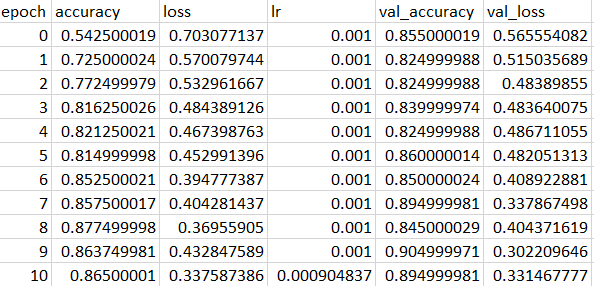
\includegraphics[width=0.6\linewidth]{Images/training_log.png}
    \caption{Snapshot of Training Log}\
    \label{fig:TrainingLog}
\end{figure}

\clearpage

\begin{itemize}
    \item ModelCheckpoint: helps to keep checkpoints at a specific training point which helps to recover that point if subsequent training gets halted by some unforeseen circumstances. This is useful when training a large model or when there is a need to add more information to an existing model.

    \item ReduceLROnPlateau: Changes the learning rate when the specified metric (here, validation loss) is not improving. Learning Rate changes at the end of the previous epoch

    \item EarlyStopping: Used to stop training when the specified metric (here, validation loss) goes out of range (means, the training curve and validation curve go away from each other)

    \item CSVLogger: Stores a piece of training information like epoch count, training accuracy, testing accuracy, training loss, and validation loss onto a CSV file. Figure \ref{fig:TrainingLog} is a snapshot of CSVLogger which shows how the results are arranged in the Comma Separated File (CSV) file.    
\end{itemize}




\noindent $\bullet$ Learning Rate Scheduler: Keeps specified initial learning rate for the first five epochs (in this case) and then it will make changes to the learning rate. Learning Rate is changed at the beginning of the current epoch.

\begin{lstlisting}
def scheduler(epoch, lr):
    if epoch < 5:
        return lr
    else:
        return lr * tf.math.exp(-0.1)
lr_scheduler = LearningRateScheduler(scheduler)
\end{lstlisting}

% \lfoot{\textit{Departmant of Artificial Intelligence and Data Science, SJCET Palai}}
% \renewcommand{\footrulewidth}{0.4pt}